\documentclass[11pt,a4paper]{article}

\usepackage[utf8]{inputenc}
\usepackage[T1]{fontenc}
\usepackage[spanish,es-tabla]{babel}
\usepackage{graphicx}
\usepackage{amsmath}
\usepackage{geometry}
\usepackage{float}
\usepackage{icomma}

\geometry{left=2.5cm, right=2.5cm, top=2.2cm, bottom=2.2cm}

\begin{document}
	
	\section*{2.3. Diseño Libre: Amplificador de Transadmitancia}
	
	\subsection*{1. Diseño del circuito y cálculos teóricos}
	Para la parte de diseño libre hemos montado el \textbf{amplificador de transadmitancia} (conversor tensión-corriente) con carga conectada a masa que aparece en las diapositivas de teoría (Figura \ref{fig:esquema}).
	
	\vspace{0.2cm}
	\begin{figure}[H]
		\centering
		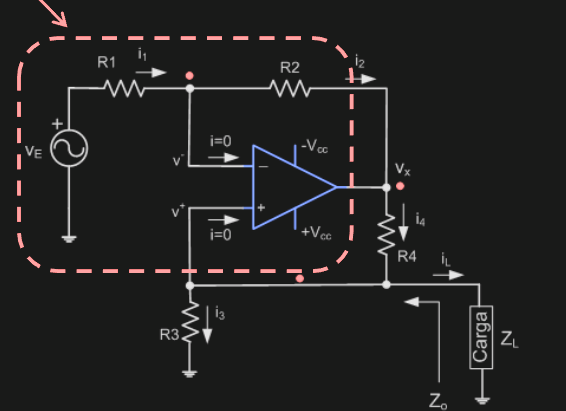
\includegraphics[width=0.55\textwidth]{esquema.png}
		\caption{Esquema del amplificador de transadmitancia con carga a masa.}
		\label{fig:esquema}
	\end{figure}
	
	El objetivo de este circuito es funcionar como una fuente de corriente controlada por tensión, es decir, que por la carga $Z_L$ circule una corriente $i_L$ proporcional a la tensión de entrada $v_E$ e independiente del valor óhmico de la carga. Resolviendo los nodos del circuito ideal, la expresión general de la corriente de salida es:
	\begin{equation}
		i_L = -\left(\frac{R_2}{R_1 \cdot R_4}\right) v_E + v_L\left(\frac{R_2}{R_1 \cdot R_4} - \frac{1}{R_3}\right)
		\label{eq:general}
	\end{equation}
	
	Para que el segundo término se anule y la corriente $i_L$ no dependa de la tensión en la carga $v_L$, se tiene que cumplir la condición de equilibrio:
	\begin{equation}
		\frac{R_2}{R_1} = \frac{R_4}{R_3}
		\label{eq:equilibrio}
	\end{equation}
	
	En nuestro montaje de laboratorio hemos utilizado tres resistencias de $220\text{ }\Omega$ y una de $120\text{ }\Omega$:
	\begin{equation}
		R_1 = 120\text{ }\Omega \quad ; \quad R_2 = R_3 = R_4 = 220\text{ }\Omega
	\end{equation}
	
	Comprobando las relaciones con estos valores vemos que:
	\begin{equation}
		\frac{R_2}{R_1} = \frac{220}{120} \approx 1,83 \quad \neq \quad \frac{R_4}{R_3} = \frac{220}{220} = 1
	\end{equation}
	
	Al ser $R_1$ distinta de $R_2$, la condición de equilibrio no se cumple exactamente, quedando la ecuación del circuito como:
	\begin{equation}
		i_L = -\frac{v_E}{120\text{ }\Omega} + \frac{v_L}{264\text{ }\Omega}
		\label{eq:real}
	\end{equation}
	
	Si hacemos $i_L = v_L/R_L$ en (\ref{eq:real}) y despejamos, queda:
	\begin{equation}
		v_L = -\,2,2\; v_E\,\frac{R_L}{264\text{ }\Omega - R_L}
		\label{eq:vl}
	\end{equation}
	Según esto, para $R_L < 264\text{ }\Omega$ la salida debería estar invertida respecto a la entrada, y cuando $R_L$ se acerca a $264\text{ }\Omega$ la ganancia crece sin límite (la realimentación positiva pasa a ser mayor que la negativa y el operacional se satura).
	
	Como hemos elegido resistencias de valores bajos y aplicamos una señal de entrada de unos $4\text{ V}$ de pico, hay que comprobar si el operacional puede dar lo que el circuito le pide. La corriente $i_1=(v_E-v_L)/R_1$ que entra por $R_1$ circula también por $R_2$, y por $R_4$ circula $i_1\,R_2/R_4=i_1$. Ambas las suministra la salida del operacional, de modo que
	\begin{equation}
		i_{op}=\frac{2\,(v_E-v_L)}{R_1}\,, \qquad v_o=v_L-\frac{R_2}{R_1}\,(v_E-v_L)
		\label{eq:iop}
	\end{equation}
	Con $v_L\approx 0$ (carga pequeña) y $v_E=4,2\text{ V}$ resulta $i_{op}=\frac{2\cdot 4,2\text{ V}}{120\text{ }\Omega}=70\text{ mA}$ y $|v_o|=1,83\cdot 4,2\text{ V}\approx 7,7\text{ V}$. Como la salida está invertida, $v_E-v_L$ crece al aumentar $R_L$ y estos valores son un mínimo. Según la hoja de características del $\mu$A741, la corriente de cortocircuito de salida es de $\pm 25\text{ mA}$ como mínimo y $\pm 40\text{ mA}$ típica, y la excursión de salida garantizada es de $\pm 10\text{ V}$ (típica $\pm 13\text{ V}$). Por tanto, con $v_E=4,2\text{ V}$ el operacional trabaja limitado en corriente, y la mayor parte del rango de $R_L$ también en tensión, así que no se puede esperar que se cumpla la ecuación (\ref{eq:vl}). Para no superar los $25\text{ mA}$ con $R_L\to0$ haría falta $v_E\le \frac{25\text{ mA}\cdot 120\text{ }\Omega}{2}=1,5\text{ V}$ de pico.
	
	\clearpage
	
	\subsection*{2. Montaje en la protoboard}
	Montamos el operacional LM741 alimentado a $\pm 15\text{ V}$ con la resistencia $R_1 = 120\text{ }\Omega$ y las tres resistencias $R_2 = R_3 = R_4 = 220\text{ }\Omega$. Con el generador de funciones metemos una señal senoidal a $1\text{ kHz}$ y unos $8\text{ Vpp}$. Pusimos un potenciómetro de hasta $10\text{ k}\Omega$ a masa como carga para poder variar $R_L$ en tiempo real sin tener que cambiar resistencias de sitio en la placa (Figura \ref{fig:montaje}).
	
	\vspace{0.2cm}
	\begin{figure}[H]
		\centering
		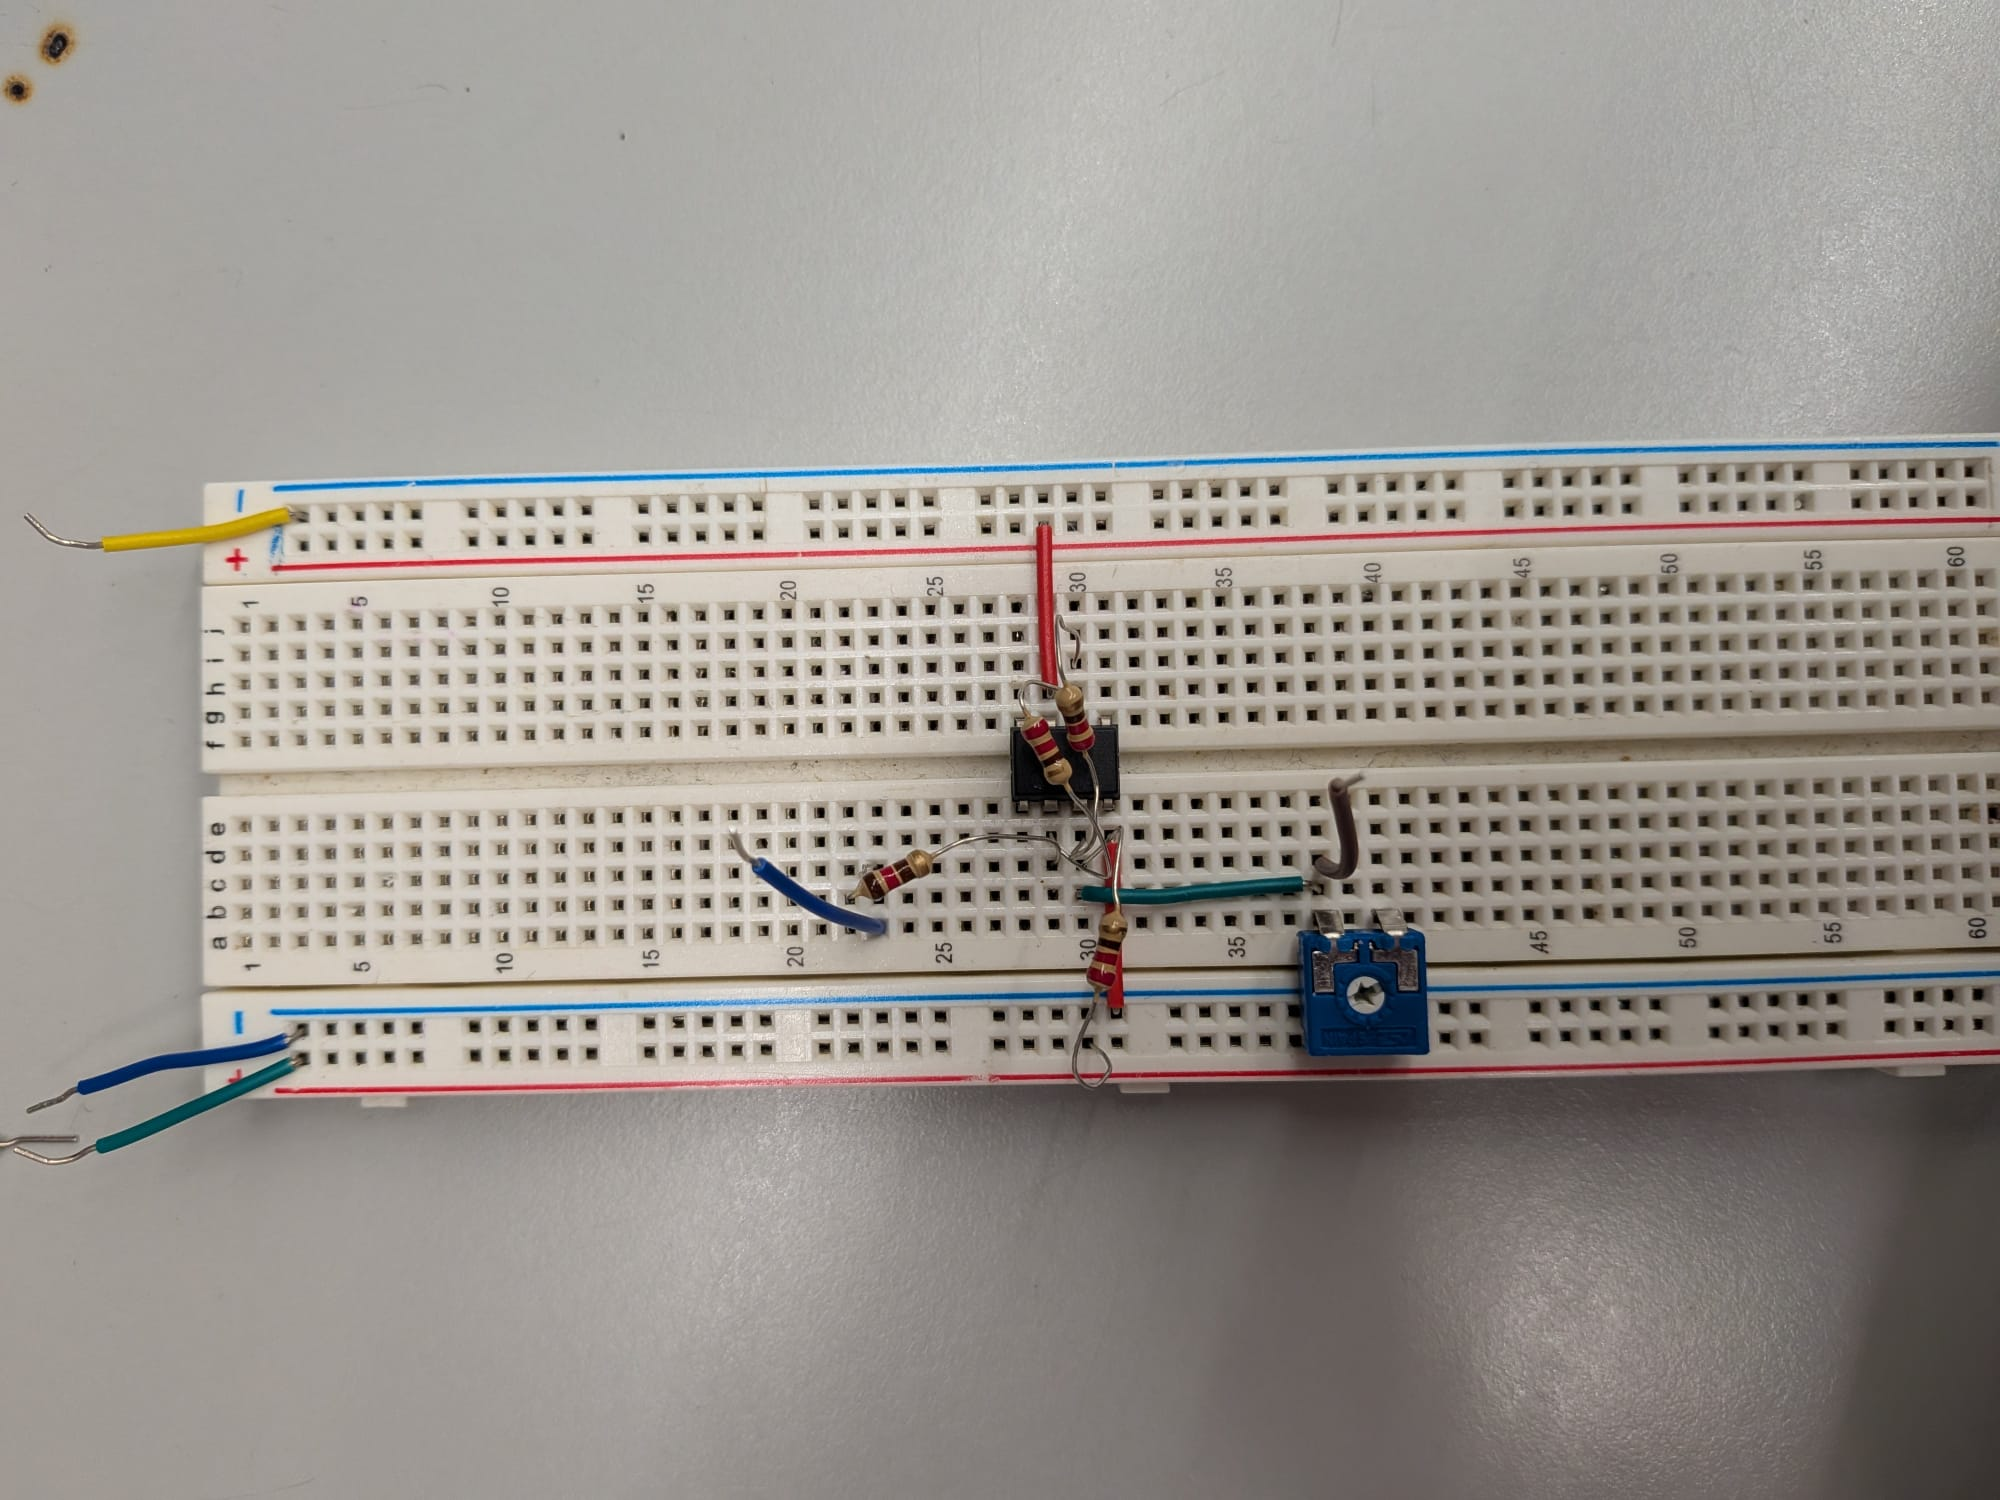
\includegraphics[width=0.52\textwidth]{montaje.jpg}
		\caption{Montaje en la protoboard usando el potenciómetro como carga variable.}
		\label{fig:montaje}
	\end{figure}
	
	\clearpage
	\subsection*{3. Medidas en el osciloscopio}
	En el osciloscopio conectamos el \textbf{Canal 1 (amarillo)} a la entrada del generador de funciones y el \textbf{Canal 2 (azul)} a la salida en la carga. 
	
	Las dos señales tienen escalas verticales distintas: el Canal 1 está a $\mathbf{5,00\text{ V/div}}$ y el Canal 2 lo pusimos a $\mathbf{1,00\text{ V/div}}$ para ver mejor la onda de salida. Por esa diferencia de escala la señal azul se ve más alta en pantalla aunque su tensión es menor. Como no activamos las medidas automáticas para el Canal 2, hemos medido su amplitud contando las divisiones de la cuadrícula (lectura con una incertidumbre de unos $\pm 0,2\text{ V}$):
	
	\vspace{0.3cm}
	\noindent\textbf{A. Potenciómetro con valor alto (Figura \ref{fig:osc1}):} 
	El generador entrega en el Canal 1 una señal de $8,40\text{ Vpp}$ ($4,20\text{ V}$ de amplitud de pico). En el Canal 2 la onda azul ocupa unas $5,3\text{ divisiones}$ pico a pico, que a escala $1,00\text{ V/div}$ corresponden a $5,3\text{ Vpp}$, es decir, $\mathbf{2,7\text{ V}}$ de pico.
	
	\begin{figure}[H]
		\centering
		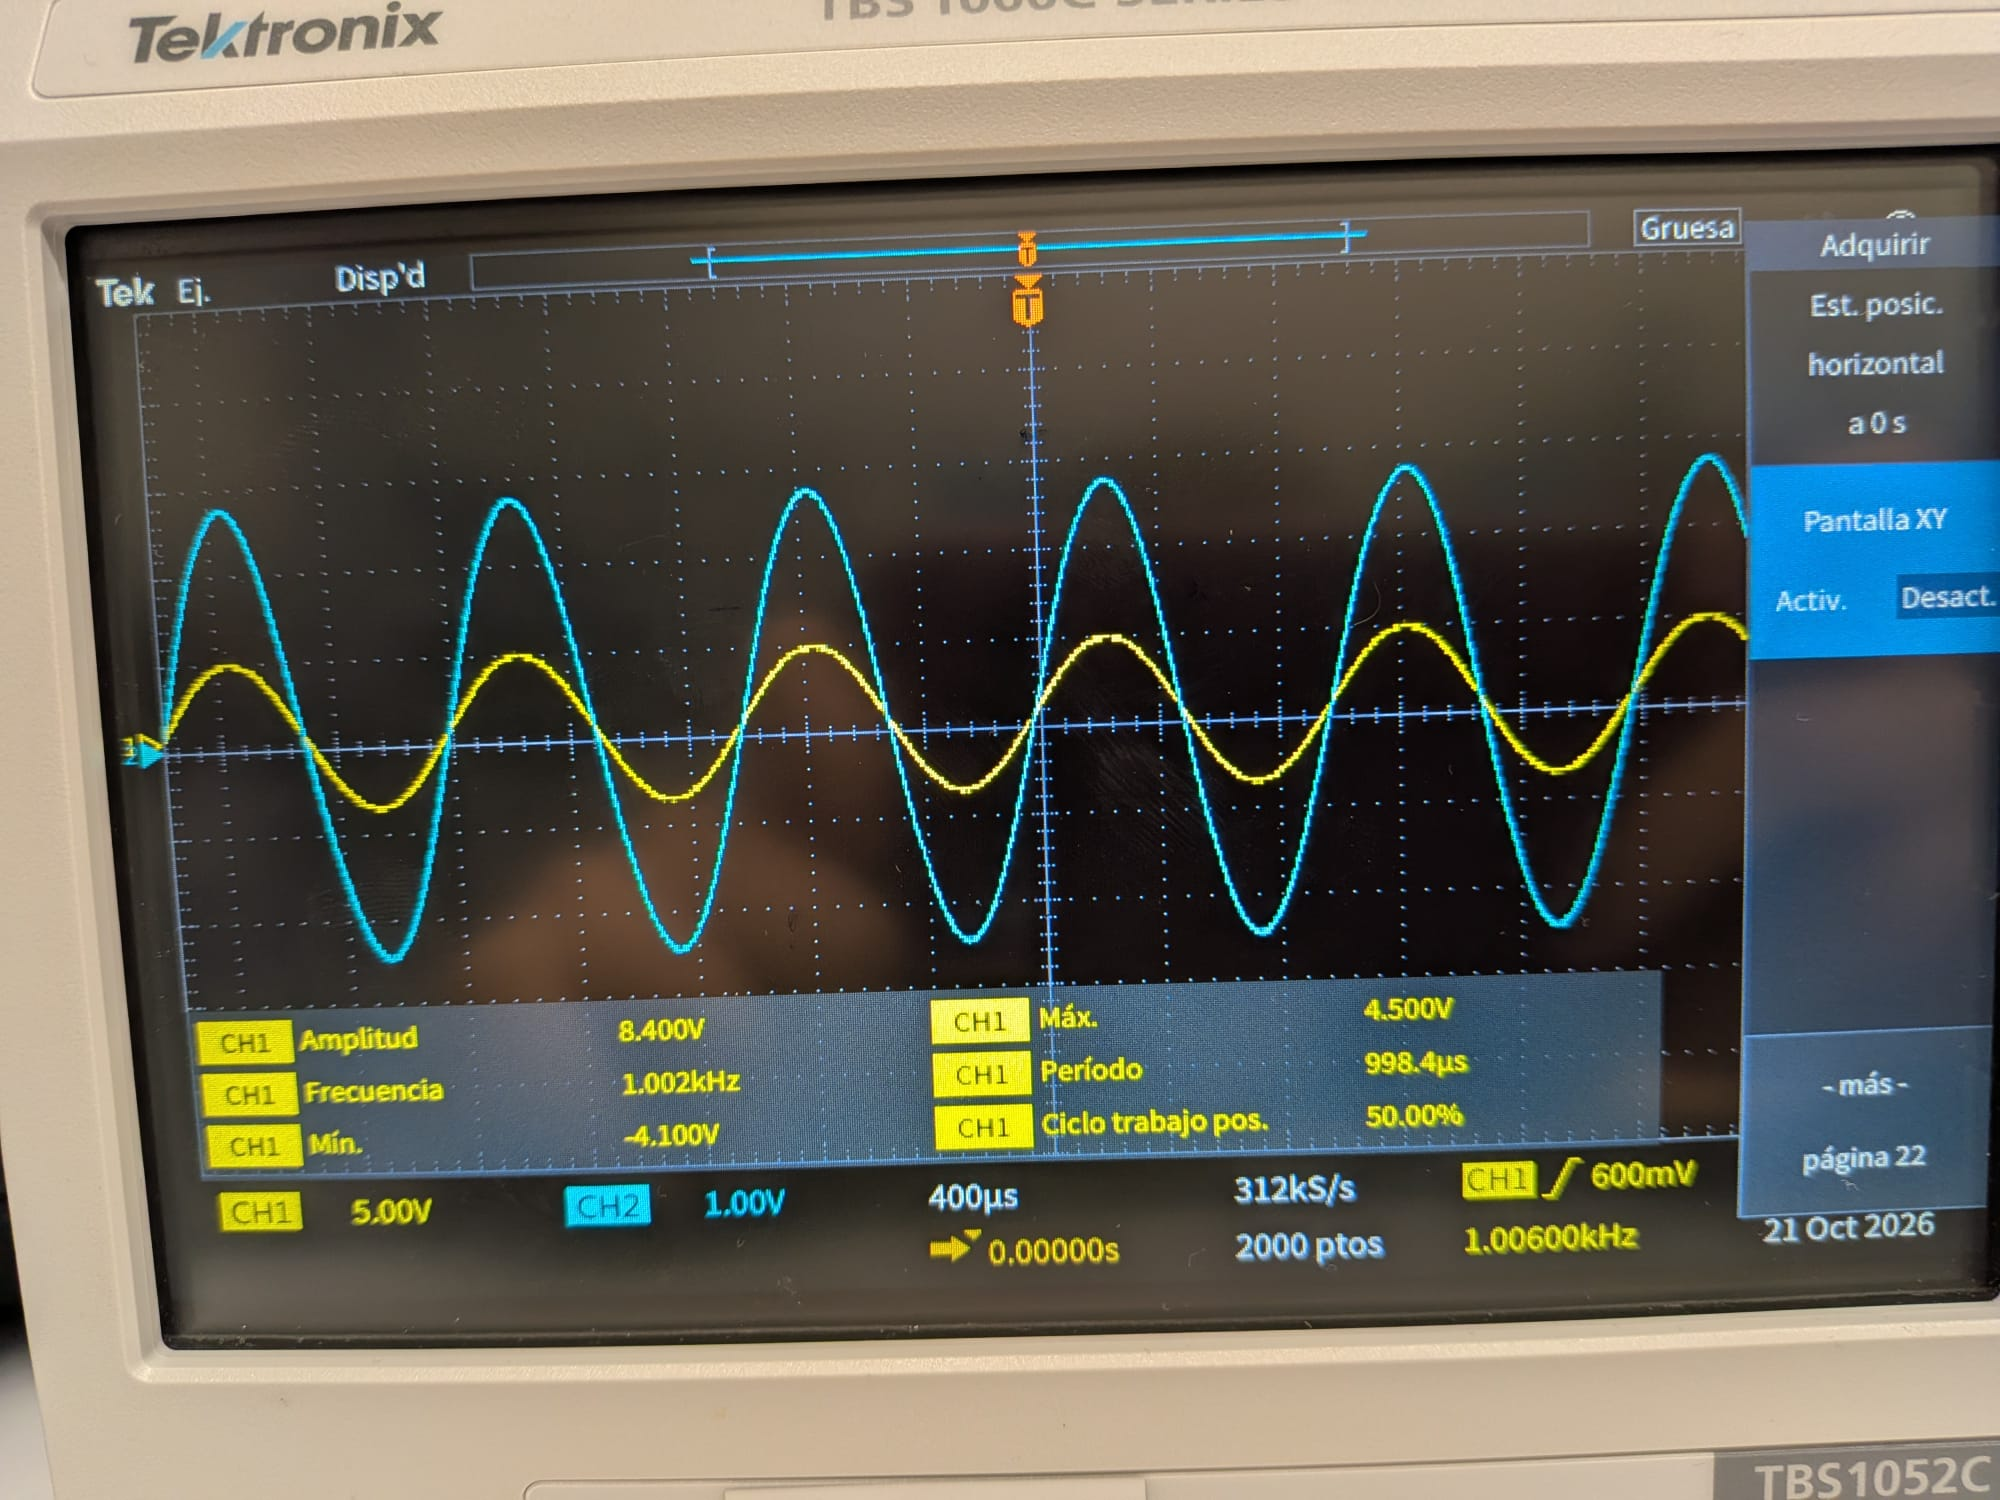
\includegraphics[width=0.48\textwidth]{osc1.jpg}
		\caption{Señal de entrada (CH1, $5\text{ V/div}$) y salida en la carga (CH2, $1\text{ V/div}$) con el potenciómetro alto.}
		\label{fig:osc1}
	\end{figure}
	
	\vspace{0.3cm}
	\noindent\textbf{B. Ajuste intermedio (Figura \ref{fig:osc2}):} 
	En esta captura giramos un poco el potenciómetro para reducir su resistencia. La entrada en el Canal 1 marca $8,00\text{ Vpp}$ ($4,00\text{ V}$ de pico) y la onda azul del Canal 2 baja hasta unas $4,2\text{ divisiones}$ pico a pico, es decir, $4,2\text{ Vpp}$ ($\mathbf{2,1\text{ V}}$ de pico).
	
	\begin{figure}[H]
		\centering
		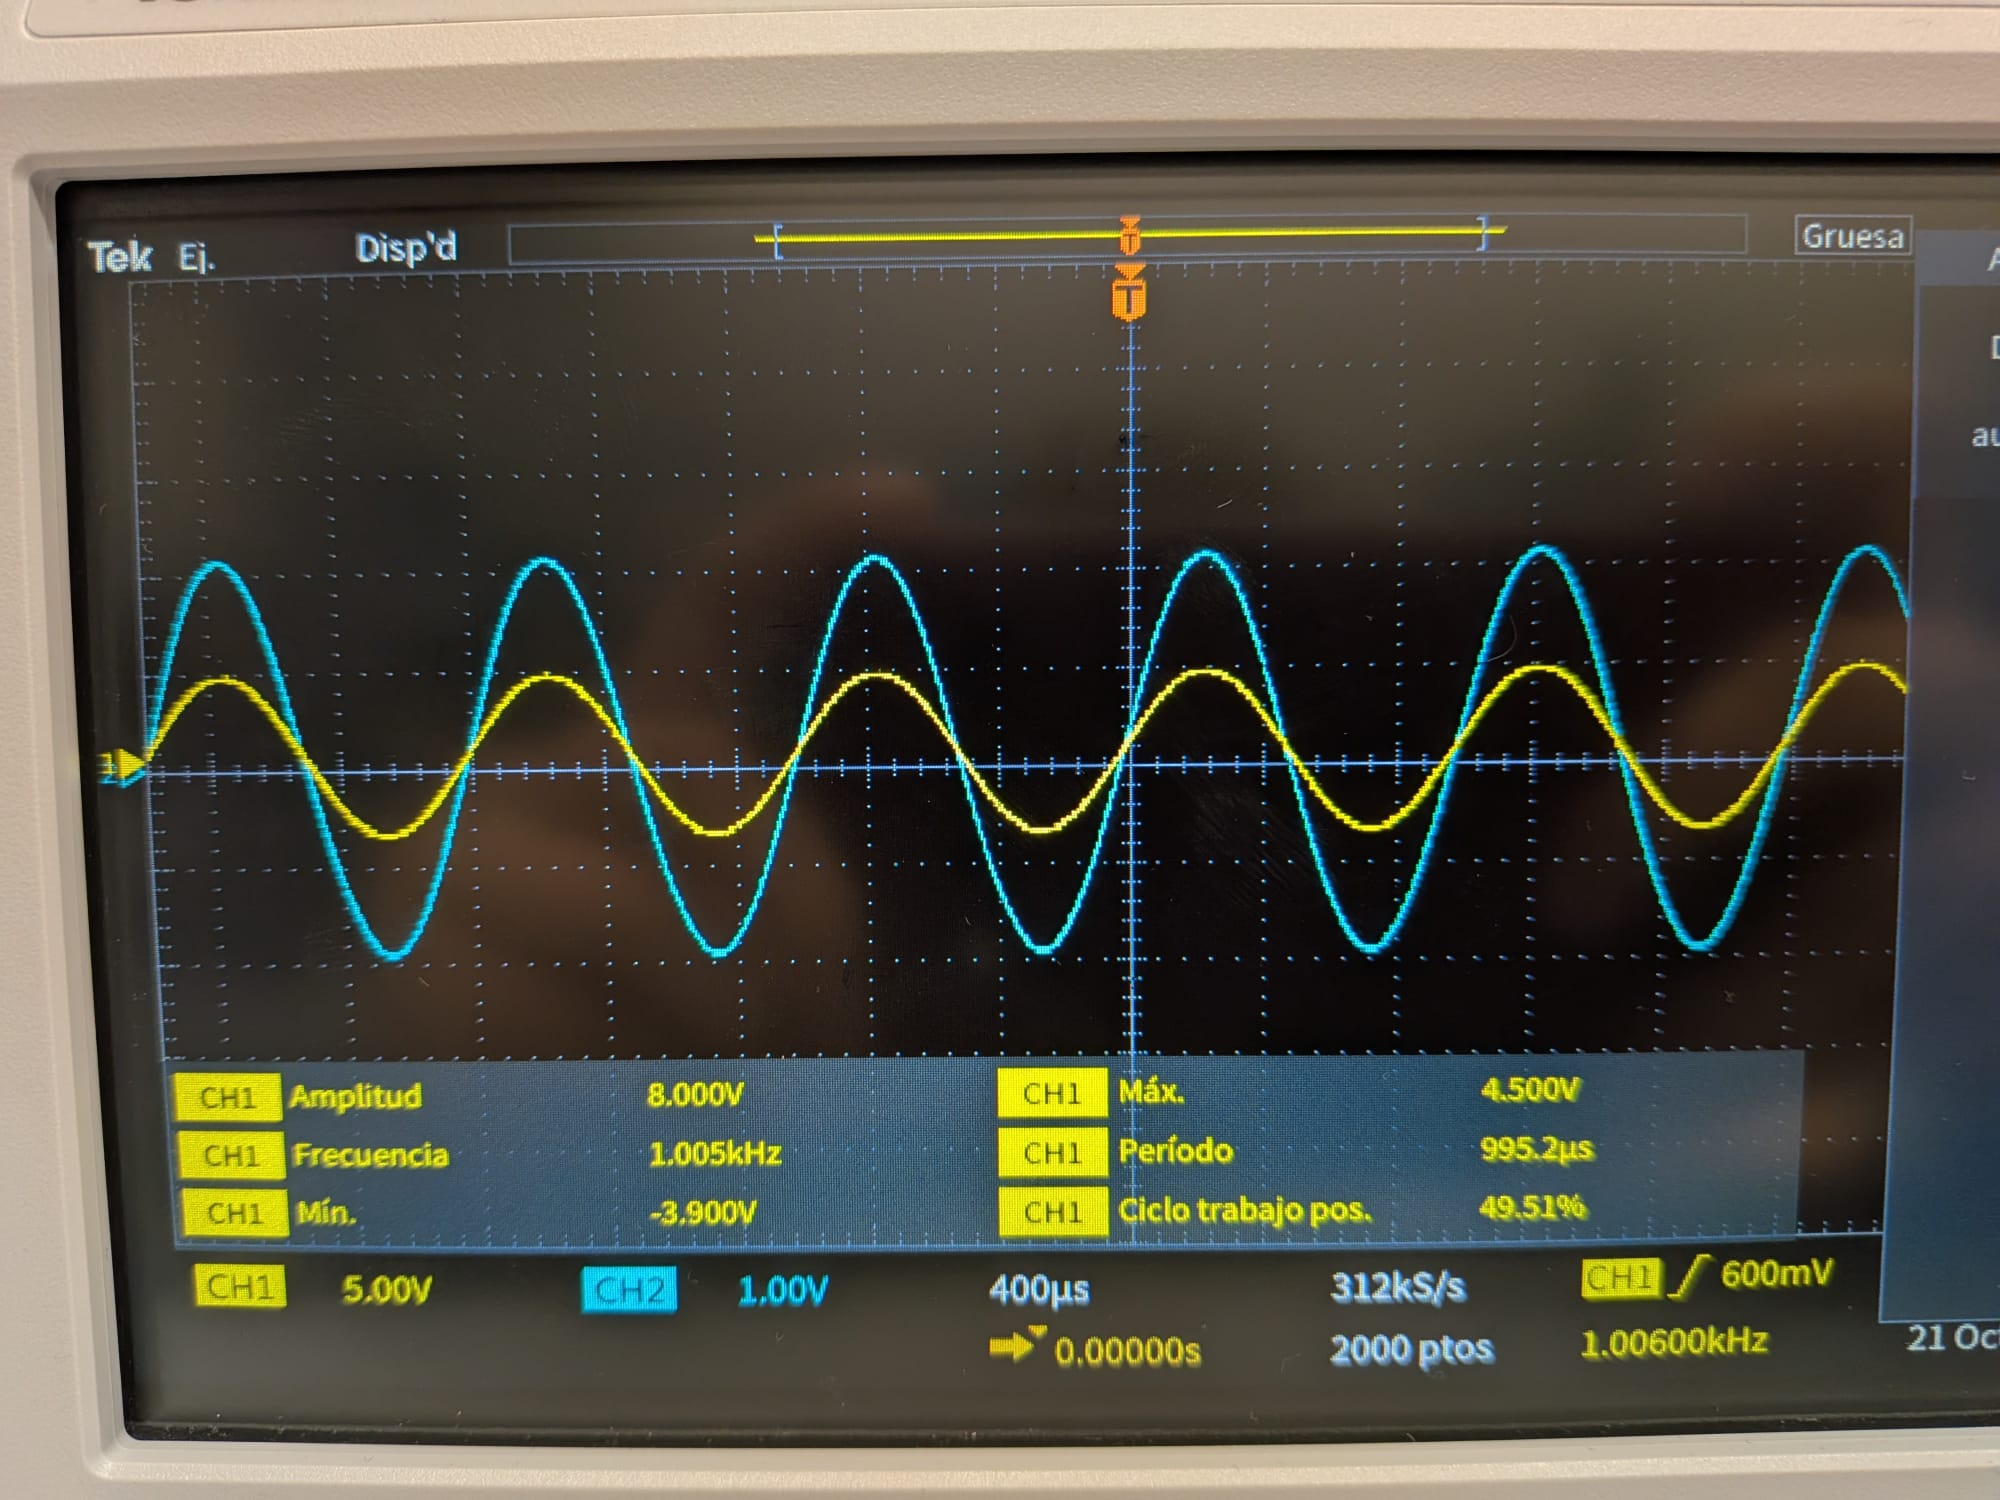
\includegraphics[width=0.48\textwidth]{osc2.jpg}
		\caption{Señales tras bajar ligeramente la resistencia del potenciómetro ($\approx 2,1\text{ V}$ de pico en CH2).}
		\label{fig:osc2}
	\end{figure}
	
	\clearpage
	\noindent\textbf{C. Potenciómetro casi al mínimo (Figura \ref{fig:osc3}):} 
	Al girar el potenciómetro casi hasta el mínimo, la tensión en el Canal 2 cae a una quinta parte de división pico a pico, unos $0,2\text{ Vpp}$ ($\mathbf{0,1\text{ V}}$ de pico), un valor comparable a la incertidumbre de lectura. También se observa que la amplitud del generador en el Canal 1 baja a $6,80\text{ Vpp}$ ($3,40\text{ V}$ de pico), probablemente por la impedancia de salida del generador al aumentar la corriente que pide el circuito.
	
	\begin{figure}[H]
		\centering
		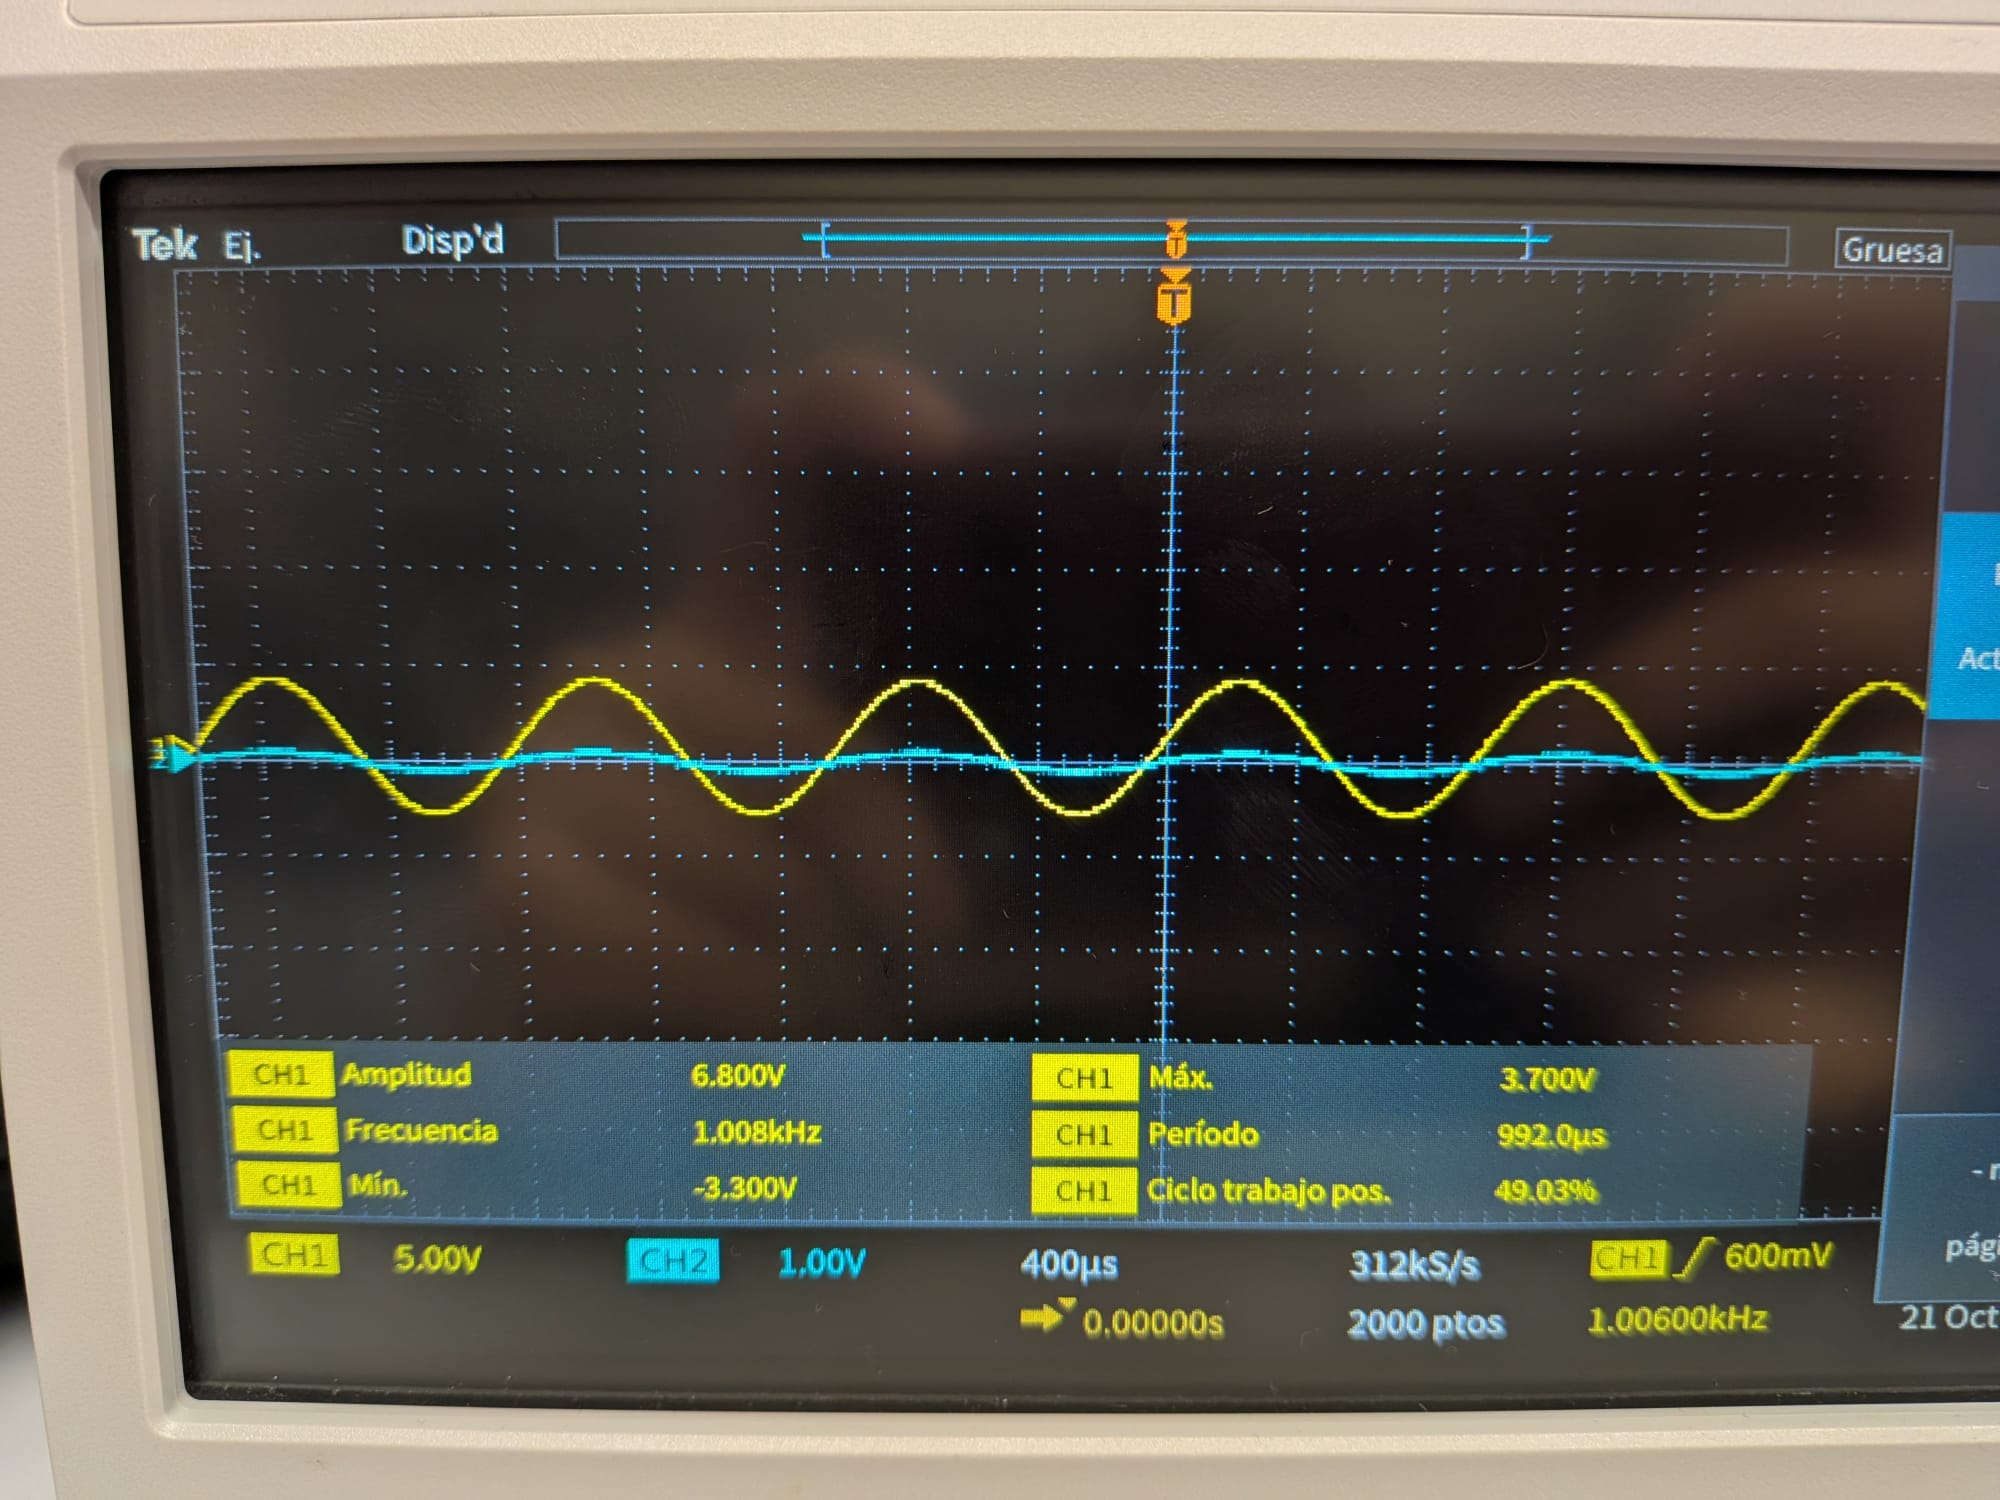
\includegraphics[width=0.48\textwidth]{osc3.jpg}
		\caption{Señales con el potenciómetro casi al mínimo.}
		\label{fig:osc3}
	\end{figure}
	
	\vspace{0.3cm}
	\noindent\textbf{D. Comparación con el modelo.} 
	En las tres capturas la onda azul y la amarilla pasan por cero y alcanzan sus máximos a la vez, es decir, la salida está \textbf{en fase} con la entrada, mientras que la ecuación (\ref{eq:vl}) predice inversión para $R_L<264\text{ }\Omega$. Para $R_L>264\text{ }\Omega$ el modelo da una salida en fase, pero con una ganancia $|v_L/v_E|>2,2$, y las ganancias medidas son
	\begin{equation}
		\frac{v_L}{v_E}\approx\frac{2,7}{4,2}=0,64\,, \qquad \frac{2,1}{4,0}=0,53\,, \qquad \frac{0,1}{3,4}\approx0,03
	\end{equation}
	respectivamente para A, B y C. Además, usando las tensiones medidas en la ecuación (\ref{eq:iop}) se obtiene $i_{op}\approx 26\text{ mA}$, $32\text{ mA}$ y $55\text{ mA}$ en A, B y C, valores del orden o por encima del límite de $25$--$40\text{ mA}$ del operacional. Como no medimos $R_L$ en ninguna captura, no podemos hacer una comparación cuantitativa con (\ref{eq:vl}), y como el operacional trabaja en el límite de su capacidad de corriente, las tres capturas deben interpretarse de forma cualitativa: la tensión en la carga disminuye al reducir $R_L$, como corresponde a $v_L=i_L R_L$, y se anula cuando $R_L\to0$.
	
\end{document}